\documentclass[11pt]{beamer}
\usetheme{Madrid}
\usecolortheme{default}
\usepackage[utf8]{inputenc}
\usepackage{graphicx}
\usepackage{caption}
\usepackage{subcaption}
\usepackage{hyperref}
\usepackage{amsmath,amssymb}
\usepackage{booktabs}
\usepackage{algorithm}
\usepackage{algorithmic}
\usepackage{xpatch}

\makeatletter
\xpatchcmd{\itemize}
  {\def\makelabel}
  {%
    \ifnum\@itemdepth=1\relax
      \setlength\itemsep{3ex}% first level
    \else\ifnum\@itemdepth=2\relax
      \setlength\itemsep{1.5ex}% second level
    \else
      \ifnum\@itemdepth=3\relax
        \setlength\itemsep{1ex}% third level
      \fi
    \fi\fi
    \def\makelabel
  }
  {}{}
\makeatother

\title{Exploring Classifier-Free Guidance}
\subtitle{ Introduction to Machine Learning Final Project}
\author{Dhruman Gupta \and Rushil Gupta}
\date{\today}

\begin{document}

\begin{frame}
  \titlepage
\end{frame}

\AtBeginSection[]
{
  \begin{frame}
    \frametitle{Table of Contents}
    \tableofcontents[currentsection]
  \end{frame}
}


\section{Motivation \& Conditioning}
\begin{frame}{Motivation}
  \begin{itemize}
    \item In the past few years, diffusion models have gained popularity as a powerful generative modeling technique.
    \item These models can be trained on samples from a distribution and can generate new samples from that distribution.
    \begin{itemize}
      \item So, given $D \sim P(x)$, we can sample $x_0 \sim P(x)$
    \end{itemize}
    \item However, a natural question, and a key challenge, is can we sample from the conditional distribution $p(x_0\mid y)$?
  \end{itemize}
\end{frame}

\begin{frame}{Applications of Conditional Generation}
  If we are able to sample from the conditional distribution, we can do a lot of things:
  \begin{itemize}
    \item Text to Image / Video Generation
    \item Text to Audio Generation
    \item Image Inpainting / Restoration
  \end{itemize}
\end{frame}

\section{Background}
\begin{frame}{Background: Diffusion Models}
  \begin{itemize}
    \item Diffusion models are a class of generative models that iteratively add noise to data and then learn to reverse this process.
    \item Idea: add noise to an image, then learn to reverse the noise process to generate images.
  \end{itemize}
\end{frame}

\begin{frame}{Forward Process}
  \begin{itemize}
    \item The forward process of adding noise is defined as:
      \[
        q(x_t \mid x_{t-1})
        = \mathcal{N}\bigl(x_t;\,\sqrt{1-\beta_t}\,x_{t-1},\,\beta_t I\bigr),
        \quad t=1,\dots,T.
      \]
      Where $x_0$ is the original image, $x_T$ is pure noise, and $\beta_t$ is a variance schedule.
    \item In the reverse process, we want to learn $p(x_{t-1}\mid x_t)$.
    \begin{itemize}
      \item If we are able to, then we can sample $x_T \sim \mathcal{N}(0, 1)$ and then iteratively sample from $p(x_{t-1}\mid x_t)$ to get $x_0$.
    \end{itemize}
  \end{itemize}
\end{frame}

\begin{frame}{Reverse Process}
  \begin{itemize}
    \item Learn to reverse noising via a neural network:
      \[
        p_\theta(x_{t-1}\mid x_t)
        = \mathcal{N}\bigl(x_{t-1};\,\mu_\theta(x_t,t),\,\sigma_t^2 I\bigr).
      \]
    \item Using score prediction, parameterize mean directly:
      \[
        \mu_\theta(x_t,t)
        = x_t + \sigma_t^2 s_\theta(x_t,t),
      \]
      where $s_\theta(x_t,t)$ is the neural network that predicts the score function $\nabla_{x_t}\log p(x_t)$.
  \end{itemize}
\end{frame}

\begin{frame}{Training Objective}
  \begin{itemize}
    \item Score matching loss:
      \[
        \mathcal{L}(\theta)
        = \mathbb{E}_{x_0,t}
          \Bigl[\|s_\text{true}(x_t, x_0, t) - s_\theta(x_t,t)\|^2\Bigr],
      \]
      where $x_t = \sqrt{\bar\alpha_t}\,x_0 + \sqrt{1-\bar\alpha_t}\,\epsilon$.
    \item This means the network $s_\theta$ directly learns to predict the score of the noisy distribution.
  \end{itemize}
\end{frame}

\begin{frame}[fragile]{Unconditional Sampling Algorithm}
  \begin{algorithmic}[1]
    \STATE $x_T \sim \mathcal{N}(0,I)$
    \FOR{$t = T, \dots, 1$}
      \STATE $s \gets s_\theta(x_t,t)$ \COMMENT{Neural network predicts score directly}
      \STATE $\mu \gets x_t + \sigma_t^2 s$
      \STATE $x_{t-1}\sim \mathcal{N}(x_{t-1};\,\mu,\sigma_t^2 I)$
    \ENDFOR
    \STATE \textbf{return} $x_0$
  \end{algorithmic}
\end{frame}

\section{Classifier Guidance}
\begin{frame}{Classifier Guidance: Concept}
  \begin{itemize}
    \item Now, we have a model that can generate samples from $p(x_0)$.
    \item We want to be able to sample from $p(x_0\mid y)$.
    \item How do we do that?
  \end{itemize}
\end{frame}

\begin{frame}{Classifier Guidance: Concept}
  \begin{itemize}
    \item Let's say we want to sample from $p(x_0\mid y)$.
    \item Update the reverse process to calculate the score of the condition $y$:
      \[
        \nabla_{x_t}\log p(x_t)
        \rightarrow \nabla_{x_t}\log p(x_t\mid y)
      \]
      \[
        \nabla_{x_t}\log p(x_t\mid y)
        = \nabla_{x_t}\log p(x_t)
        + \nabla_{x_t}\log p(y\mid x_t).
      \]
    \item The first term is exactly what diffusion models do. The second term is the score of the condition.
  \end{itemize}
\end{frame}

\begin{frame}{Classifier Guidance: Math}
  \begin{itemize}
    \item How do we get the $\nabla_{x_t}\log p(y\mid x_t)$ term?
    \item We can train a classifier $p_\phi(y\mid x_t)$ to predict the condition $y$ given the noisy image $x_t$.
    \item This was state-of-the-art in 2021, and significantly improved the quality of generated samples.
  \end{itemize}
\end{frame}

\section{Classifier‐Free Guidance}
\begin{frame}{Classifier-Free Guidance: Idea}
  \begin{itemize}
    \item Having an auxiliary classifier is not always feasible, and it can lead to instability and mode collapse.
    \item We want to be able to have a more harmonious model that can be steered by a condition.
    \item How can we have an entirely generative model do this?
  \end{itemize}
\end{frame}

\begin{frame}{Classifier‐Free Guidance: Concept}
  \begin{itemize}
    \item Recall, our goal is to estimate $\nabla_{x_t}\log p(x_t\mid y)$.
    \item Currently, our model learns $\nabla_{x_t}\log p(x_t)$.
    \item This is the same as conditioning on nothing: $\nabla_{x_t}\log p(x_t\mid \varnothing)$.
    \item So our unconditional model is actually a special case of a conditional model.
  \end{itemize}
\end{frame}

\begin{frame}{Classifier‐Free Guidance: Concept}
  \begin{itemize}
    \item Let $s_\theta(x_t,t,c) \approx \nabla_{x_t}\log p(x_t\mid c)$.
    \item Train the diffusion model to predict both:
      \[
      s_\theta(x_t,t,c)
      \quad\text{and}\quad
      s_\theta(x_t,t,\varnothing)
      \]
      by randomly dropping the condition $c$ during training.
    \item At inference, combine:
      \[
      s_{\mathrm{CFG}}
      = (1+w)\,s_\theta(x_t,t,c)
      - w\,s_\theta(x_t,t,\varnothing),
      \]
      where $w$ is the guidance weight.
    \item \textbf{Advantage:} no extra classifier, single unified model.
    \end{itemize}
  \end{frame}

\begin{frame}[fragile]{CFG Sampling Algorithm}
  \begin{algorithmic}[1]
    \STATE $x_T \sim \mathcal{N}(0,I)$
    \FOR{$t = T, \dots, 1$}
      \STATE $s_c \gets s_\theta(x_t,t,c)$
      \STATE $s_u \gets s_\theta(x_t,t,\varnothing)$ 
      \STATE $s \gets (1+w)\,s_c - w\,s_u$ 
      \STATE $\mu \gets x_t + \sigma_t^2 s$
      \STATE $x_{t-1}\sim \mathcal{N}(x_{t-1};\,\mu,\sigma_t^2 I)$
    \ENDFOR
    \STATE \textbf{return} $x_0$
  \end{algorithmic}
\end{frame}

\section{Implementation \& Training}
\begin{frame}{Implementation Overview}
  \begin{itemize}
    \item We used the pre-trained VAE from stable diffusion v1.4 to encode and decode images.
    \item We used the pre-trained CLIP text encoder to encode the text prompts.
    \item The diffusion model is a UNet with 4 down/up blocks and 960 channels.
  \end{itemize}
\end{frame}

\begin{frame}{What Is a UNet?}
  \begin{itemize}
    \item \textbf{Purpose:}  
      \begin{itemize}
        \item Designed for image-to-image tasks (e.g., denoising, segmentation).
        \item Learns to reverse a corruption process by progressively refining features.
      \end{itemize}
    \item \textbf{Key Idea:}  
      \begin{itemize}
        \item Combines high‑resolution spatial information with deep, coarse features.
        \item The idea is to capture both local and global context.
      \end{itemize}
    \item \textbf{Origin:}  
      \begin{itemize}
        \item First introduced for biomedical image segmentation (Ronneberger et al., 2015).
      \end{itemize}
  \end{itemize}
\end{frame}

\begin{frame}{UNet Architecture Overview}
  \begin{itemize}
  \item \textbf{Encoder (Contracting Path):}
    \begin{itemize}
      \item Stacks of Conv$\rightarrow$ReLU$\rightarrow$Conv$\rightarrow$ReLU.
    \end{itemize}
  \item \textbf{Bottleneck:}
    \begin{itemize}
      \item deepest layer; captures the most abstract features.
      \item No pooling—just convolutions.
    \end{itemize}
  \item \textbf{Decoder (Expanding Path):}
    \begin{itemize}
      \item Upsamples (transposed conv) to restore spatial size, halves channels each step.
    \end{itemize}
  \item \textbf{Skip Connections:}
    \begin{itemize}
      \item Concatenate encoder feature maps to decoder at each level.
      \item Preserve fine-grained details lost during downsampling.
    \end{itemize}
\end{itemize}
\end{frame}

\begin{frame}{UNet Architecture Overview}
  \begin{figure}[ht]
  \centering
  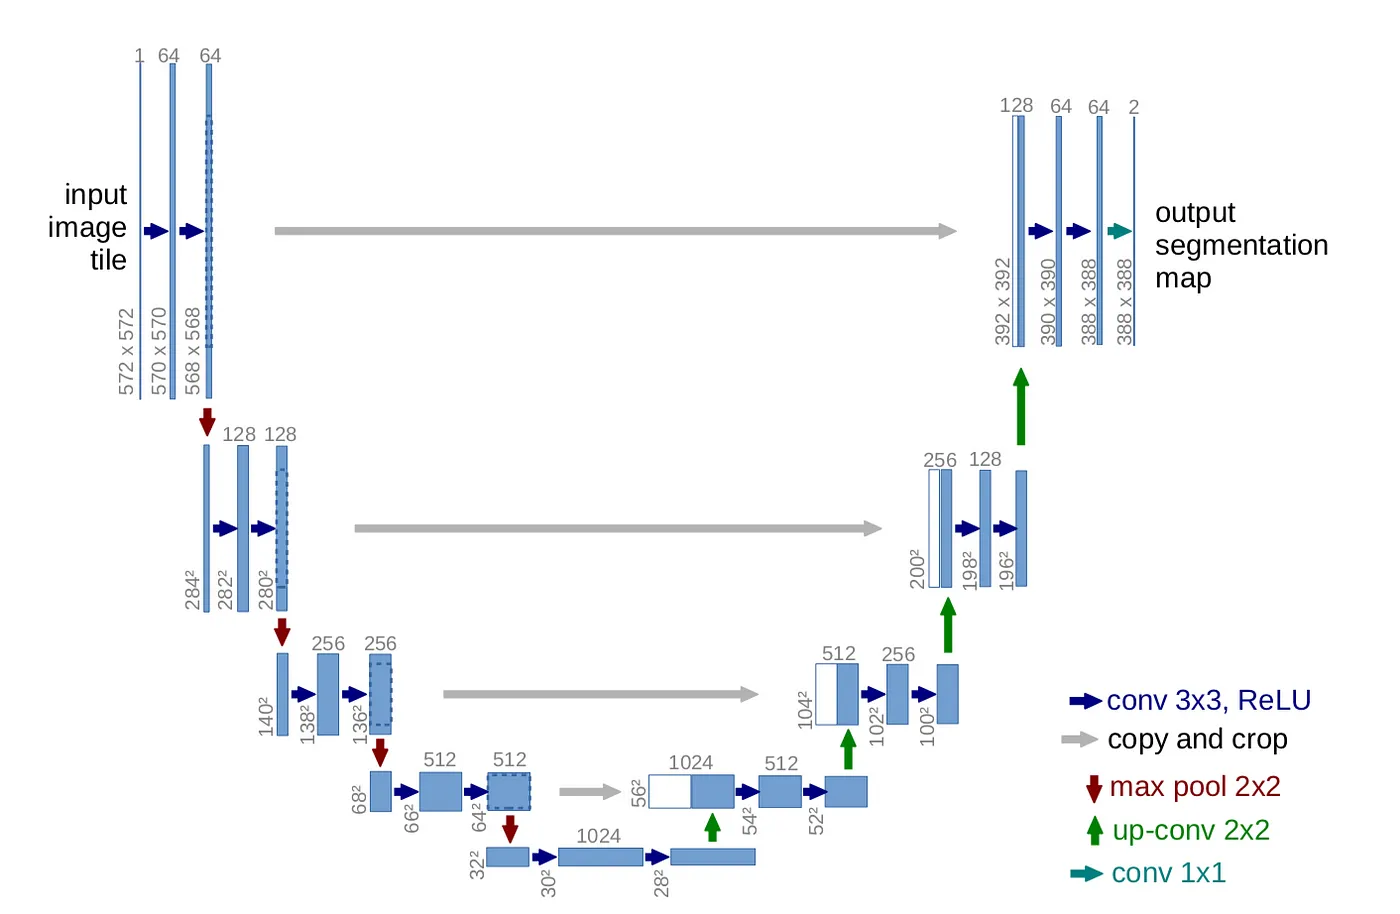
\includegraphics[width=0.85\textwidth]{figures/unet.png}
  \caption{UNet Architecture}
  \end{figure}
\end{frame}


\begin{frame}{Data Pipeline \& Caption Dropout}
  \begin{itemize}
    \item Dataset: MS COCO 2014 captions
    \begin{itemize}
      \item Contains 200K images having annotations for object detection, segmentation, and captioning
      \item Comprises of 80 categories including common objects like cars, bicycles, and animals, as well as more specific categories such as umbrellas, handbags, and sports equipment
    \end{itemize}
    \item Images resized to $128\times128$ and center-cropped
  \end{itemize}
\end{frame}

\begin{frame}{Training Details}
  \begin{itemize}
    \item The diffusion model's process is set to $1000$ timesteps.
    \item Training consisted of $450$ epochs.
  \end{itemize}
\end{frame}

\begin{frame}{Inference \& Sampling}
  \begin{itemize}
    \item Sweep guidance weights $w \in \{1,3,5,7\}$
    \item Fixed seed for consistent comparisons
    \item Generate 3×3 grids per prompt and weight
  \end{itemize}
\end{frame}

\section{Results}
\begin{frame}{Results}
  \begin{itemize}
    \item We train the model for 450 epochs.
    \item Results are not the most impressive, since we are using a small model and dataset - due to compute constraints.
  \end{itemize}
\end{frame}

\begin{frame}{Results - Snowy Mountain}
    \begin{figure}
      \centering
      \begin{subfigure}[b]{0.24\textwidth}
        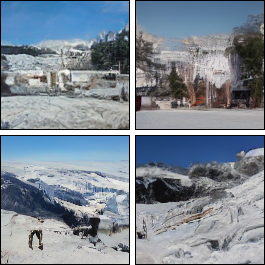
\includegraphics[width=\linewidth]{figures/a_beautiful_snowy_mountain_landscape_1.png}
        \caption{$w=1.0$}
      \end{subfigure}
      \begin{subfigure}[b]{0.24\textwidth}
        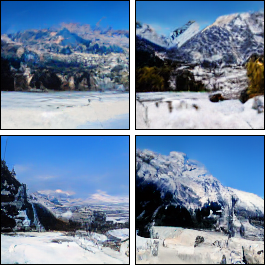
\includegraphics[width=\linewidth]{figures/a_beautiful_snowy_mountain_landscape_3.png}
        \caption{$w=3.0$}
      \end{subfigure}
      \vspace{0.5em}
      \begin{subfigure}[b]{0.24\textwidth}
        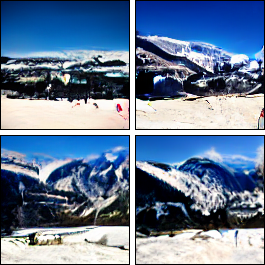
\includegraphics[width=\linewidth]{figures/a_beautiful_snowy_mountain_landscape_5.png}
        \caption{$w=5.0$}
      \end{subfigure}
      \begin{subfigure}[b]{0.24\textwidth}
        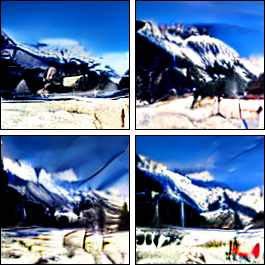
\includegraphics[width=\linewidth]{figures/a_beautiful_snowy_mountain_landscape_7.png}
        \caption{$w=7.0$}
      \end{subfigure}
      \caption{"a beautiful snowy mountain landscape" with different guidance weights}
    \end{figure}
  \end{frame}

  \begin{frame}{Results - Beach}
    \begin{figure}
      \centering
      \begin{subfigure}[b]{0.24\textwidth}
        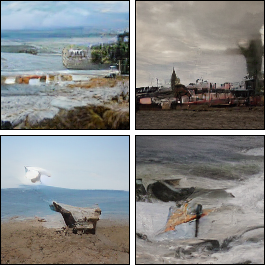
\includegraphics[width=\linewidth]{figures/a_beach_1.png}
        \caption{$w=1.0$}
      \end{subfigure}
      \begin{subfigure}[b]{0.24\textwidth}
        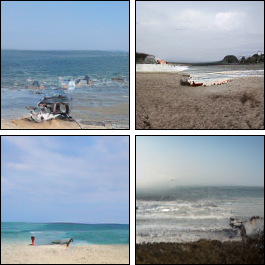
\includegraphics[width=\linewidth]{figures/a_beach_3.png}
        \caption{$w=3.0$}
      \end{subfigure}
      \vspace{0.5em}
      \begin{subfigure}[b]{0.24\textwidth}
        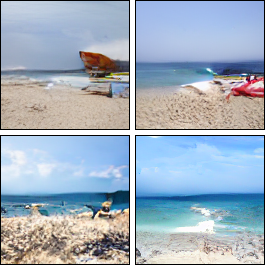
\includegraphics[width=\linewidth]{figures/a_beach_5.png}
        \caption{$w=5.0$}
      \end{subfigure}
      \begin{subfigure}[b]{0.24\textwidth}
        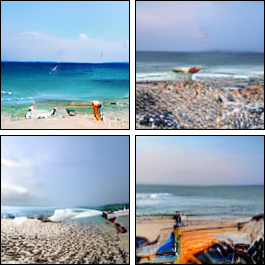
\includegraphics[width=\linewidth]{figures/a_beach_7.png}
        \caption{$w=7.0$}
      \end{subfigure}
      \caption{"a beach" with different guidance weights}
    \end{figure}
  \end{frame}


\begin{frame}{Results - Tennis Court}
    \begin{figure}
      \centering
      \begin{subfigure}[b]{0.24\textwidth}
        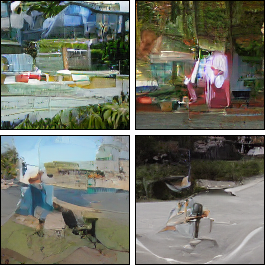
\includegraphics[width=\linewidth]{figures/A_tennis_court_1.png}
        \caption{$w=1.0$}
      \end{subfigure}
      \begin{subfigure}[b]{0.24\textwidth}
        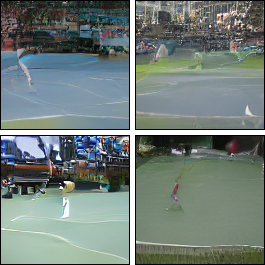
\includegraphics[width=\linewidth]{figures/A_tennis_court_3.png}
        \caption{$w=3.0$}
      \end{subfigure}
      \vspace{0.5em}
      \begin{subfigure}[b]{0.24\textwidth}
        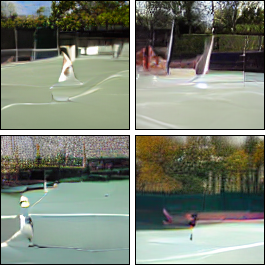
\includegraphics[width=\linewidth]{figures/A_tennis_court_5.png}
        \caption{$w=5.0$}
      \end{subfigure}
      \begin{subfigure}[b]{0.24\textwidth}
        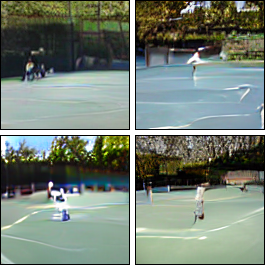
\includegraphics[width=\linewidth]{figures/A_tennis_court_7.png}
        \caption{$w=7.0$}
      \end{subfigure}
      \caption{"a tennis court" with different guidance weights}
    \end{figure}
  \end{frame}


  \section{Discussion}
\begin{frame}{Discussion}
  \begin{itemize}
    \item Increasing guidance weight enhances prompt adherence but reduces sample diversity, leading to mode collapse at high $w$.
    \item Due to our small dataset and limited model parameters, high guidance weights can introduce artifacts.
    \item Failure cases on novel objects highlight dataset limitations: COCO lacks sufficient examples of uncommon items.
    \item The chosen UNet size balances capacity and compute but may underfit complex scenes.
  \end{itemize}
\end{frame}

\section{Future Work}
\begin{frame}{Future Work}
  \begin{itemize}
    \item Expand the training corpus with larger captioned datasets (e.g., OpenImages, LAION) to improve object diversity.
    \item Use parameter-efficient fine-tuning (LoRA) to enable larger backbone models under compute constraints.
    \item Explore alternative noise schedules and fewer timesteps to accelerate training and improve image sharpness.
  \end{itemize}
\end{frame}

\section{Conclusion}
\begin{frame}{Conclusion}
  \begin{itemize}
    \item We implemented classifier‑free guidance in a custom diffusion model and systematically explored its qualitative impact.
    \item CFG offers a simple yet powerful control knob for balancing fidelity and diversity.
    \item Our findings underscore the importance of dataset scale and model capacity for reliable generative performance.
  \end{itemize}
\end{frame}

\section{Bibliography}
\begin{frame}{Bibliography}
  \bibliographystyle{plain}
  \bibliography{refs}
  \bibitem{sohl2015deep}
  Sohl-Dickstein, Jascha, Eric A. Weiss, Niru Maheswaranathan, and Surya Ganguli.
  \newblock Deep Unsupervised Learning using Nonequilibrium Thermodynamics.
  \newblock In {\em Proceedings of the 32nd International Conference on Machine Learning (ICML)}, 2015.
  
  \bibitem{ho2020denoising}
  Ho, Jonathan, Ajay Jain, and Pieter Abbeel.
  \newblock Denoising Diffusion Probabilistic Models.
  \newblock In {\em Advances in Neural Information Processing Systems (NeurIPS)}, 2020.
  
  \bibitem{dhariwal2021diffusion}
  Dhariwal, Prafulla and Alex Nichol.
  \newblock Diffusion Models Beat GANs on Image Synthesis.
  \newblock In {\em Advances in Neural Information Processing Systems (NeurIPS)}, 2021.
  
  \bibitem{ho2022classifierfree}
  Ho, Jonathan and Tim Salimans.
  \newblock Classifier-Free Diffusion Guidance.
  \newblock In {\em Advances in Neural Information Processing Systems (NeurIPS)}, 2022.
\end{frame}

\end{document}
